\documentclass{article}
\usepackage[utf8]{inputenc}

\usepackage[margin=1in]{geometry}
\usepackage{hyperref}
\usepackage{graphicx}
 \usepackage{float}

\usepackage{titlesec}
\setcounter{secnumdepth}{4}
\setcounter{tocdepth}{4}
\titleformat{\paragraph}
{\normalfont\normalsize\bfseries}{\theparagraph}{1em}{}
\titlespacing*{\paragraph}
%{0pt}{3.25ex plus 1ex minus .2ex}{1.5ex plus .2ex}
{0pt}{0.0ex plus 1ex minus .2ex}{1.0ex plus .2ex}

\newcommand{\name}{ECW\ }
\newcommand{\nameNospace}{ECW}
\newcommand{\namep}{ECW.}

\renewcommand{\labelenumii}{\theenumii}
\renewcommand{\theenumii}{\theenumi.\arabic{enumii}}
\renewcommand{\theenumiii}{\theenumii.\arabic{enumiii}}

\usepackage{fancyhdr}
\pagestyle{fancy}

\lhead{ Responsible: Alexander Ekman \& Linnea Johnsson \\ Date: \today}  \rhead{Document number: PUSS21411 \\ Version: 1.0}
\renewcommand{\headrulewidth}{0.5pt} 


 \title{SDP - Software Development Plan}
 \author{Team 1 - ETSN05}

\begin{document}
\date{}
\maketitle
\thispagestyle{fancy}
\newpage

\section*{Revision History}
\begin{table}[h]
    \centering
    \begin{tabular}{|l|l|p{55mm}|l|}
    \hline
    Date & Version & Description & Author \\ 
    \hline\hline 
    2021-09-14 & 1.0 & First draft and outlines of all sections & Linnea Johnsson \\
    \hline
    & & & \\ 
    \hline
    \end{tabular}
    \label{tab:history}
\end{table}
\newpage
 
\section*{Referenced Documents}\label{refdoc}
\begin{enumerate}
    \item Programvaruutveckling för Stora System - Projekthandledning 2021 (PH)
    \item Product Requirements Document - PUSS21412 (PRD)
    \item Software Product Features Backlog(SPF) - PUSS21413
    \item Sprint log/plan (SP) - PUSS21414
    \item Software Top Level Design Document (STLDD) - PUSS21415
    \item Software Detailed Design Document (SDD) - PUSS21416
    \item Software Verification and Validation Report (SVVR) - PUSS21417
    \item System Specification Document (SSD) - PUSS21418
    \item Project Final Report (PFR) - PUSS21419

\end{enumerate}
\newpage

\tableofcontents
\newpage

\section{Introduction}
This Software Development Plan (SDP) details the development plan produced for the development of the web-app based carpool service called ETSN05\_PG1 Carpool Webb-app (\nameNospace). The plan includes the process model with the project's different phases and their corresponding time-estimates and major events, and the tailoring of the project. The SDP also includes a description of the project's organisation, time plan, configuration handling, and quality review, as well as a a risk analysis of the project.  

\section{Process model}
The process model mostly follow the directions from the PH chapter 2. The things that differ, and/or need more explanation, are described below.
\subsection{Phases}
The project is divided into four phases, where the last three are part of sprints. All phases include milestones in the form of documents to produce, deadlines to meet and meeting to have such as the Sprint Planning Meeting (SPM) and the Reflection Meeting(RM). These two meetings will be held back to back of each other in order to ensure a high attendance. Other meetings include the Daily stand up meeting, which will be held over zoom Mondays and Fridays, and over slack on Wednesdays, Tuesdays and Thursdays. This is also to be respectful of the team members conflicting course schedules. 

The phases that includes sprints has time for development of the ECW. The phases also includes mandatory coursework requiring time from the project members, these will be excluded from this section but will be further explained in section Time Plan.
\subsubsection{Phase 1}
In table \ref{tab:phase1} the major events from the first phase are listed in order to create an easily accessible overview. 
\begin{table}[H]
    \centering
    \begin{tabular}{|c|c|c|}
    \hline
        Activity & Deadline & Responsible \\
        \hline \hline
        SDP & 2021-09-15 & PO \\
        \hline
        PRD & 2021-09-15 & PO \\
        \hline
        SPM1 & 2021-09-10 & All \\
        \hline
        SPF1 & 2021-09-10 & PO \\
        \hline
        SP1 & 2021-09-10 & SG \& UG \\
        \hline
        Review 1 & 2021-09-17 & All \\
        \hline
    \end{tabular}
    \caption{The major events occurring in phase 1}
    \label{tab:phase1}
\end{table}

\subsubsection{Phase 2}
Table \ref{tab:phase2} shows the seconds phase's main activities.
\begin{table}[H]
    \centering
    \begin{tabular}{|c|c|c|}
    \hline
        Activity & Deadline & Responsible \\
        \hline \hline
        Sprint 1 & 2021-09-26 & DG \& SG \\
        \hline
        RM & 2021-09-24 & All \\
        \hline
        Daily Stand Up & - & UG, SG, \& SM \\
        \hline
        STLD & 2021-09-29 & SG \\
        \hline
        SPM2 & 2021-09-24 & All \\
        \hline
        SPF2 & 2021-09-14 & PO \\
        \hline
        SP2 & 2021-09-14 & SG \& UG \\
        \hline
        Review 2 & 2021-10-01 & All \\
        \hline
    \end{tabular}
    \caption{The major events occurring in phase 2}
    \label{tab:phase2}
\end{table}

\subsubsection{Phase 3}
The thirds phase's major event are included in table \ref{tab:phase3}.
\begin{table}[H]
    \centering
    \begin{tabular}{|c|c|c|}
    \hline
        Activity & Deadline & Responsible \\
        \hline \hline
        Sprint 2 & 2021-10-10 & DG \& SG \\
        \hline
        RM & 2021-10-08 & All \\
        \hline
        Daily Stand Up & - & UG, SG, \& SM \\
        \hline
        SDD & 2021-10-13 & DG \\
        \hline
        SPM3 & 2021-10-08 & All \\
        \hline
        SPF3 & 2021-10-08 & PO \\
        \hline
        SP3 & 2021-10-08 & SG \& UG \\
        \hline
        Review 3 & 2021-10-15 & All \\
        \hline
    \end{tabular}
    \caption{The major events occurring in phase 3}
    \label{tab:phase3}
\end{table}

\subsubsection{Phase 4}
The last phase's major events can be viewed in table \ref{tab:phase4}, including and ending with the final review. 
\begin{table}[H]
    \centering
    \begin{tabular}{|c|c|c|}
    \hline
        Activity & Deadline & Responsible \\
        \hline \hline
        Sprint 3 & 2021-10-22 & DG \& SG \\
        \hline
        RM & 2021-10-22 & All \\
        \hline
        Daily Stand Up & - & UG, SG, \& SM \\
        \hline
        SVVR & 2021-10-22 & SG \& DG \\
        \hline
        SSD & 2021-10-22 & PO \\
        \hline
        PFR & 2021-10-22 & PO \\
        \hline
        Final Review & 2021-10-22 & All \\
        \hline
    \end{tabular}
    \caption{The major events occurring in phase 4}
    \label{tab:phase4}
\end{table}

\section{Project Organisation}
The project is organized into a Project Group (PG), Developing Group (DG), and a System Group (SG). The PG consists of the Project Owners (PO) and Scrum Master(SM), the DG consists of developers and the architects, and the SG consists soly of the architects. Within the DG there are different areas of responsibilities. There are mainly four areas of responsibilities that corresponds to three different groups, and one sole role. There is the Algorithms Group (AG), the Frontend Group (FG), and the Backend Group(BG). There is also one role responsible for testing (TR). 

Besides the above mentioned internal actors the project has an external section chief, a customer, a reviewer, and three different experts. The experts have different areas of expertise. There is one requirement expert, one test expert, and one design expert.
\subsection{Project team members}
The project's team member and their corresponding roles can be seen in table \ref{team}. All the team members are enrolled in the course ETSN05 and participating in the project for educational purposes. The members have been given their different groups and roles based on interests and experience. 
\begin{table}[h]
    \centering
    \begin{tabular}{|c|c|c|}
    \hline
        Group & Name & Role \\
        \hline \hline
        PG & Alexander Ekman & PO \\ 
        & Linnea Johnsson & PO \\
        & David Ravanelli & SM \\
        \hline
        AG & Max Fogwall & Architect \& TR \\
        & Emil Friberg & Developer \\
        & Gustav Broman & Developer \\
        \hline
        FG & Erik Kullberg & Architect \\
        & Axel Domell & Developer\\ 
        & Erik Busk & Developer \\
        & Johannes Bastmark & Developer\\
        \hline
        BG & Anton Håkansson & Developer\\
        & Elsa Lindhé & Developer\\
        & Eric Schyllert  & Developer\\
        \hline
    \end{tabular}
    \caption{The ECW project's team members}
    \label{team}
\end{table}

\section{Configuration Handling}
This project consists of several documents of different character, varying from source code to text documents such as this. There are two main libraries for the different types of configuration units. The first one is GitLab that contains the project's source code, the backlog, the sprint logs, and the SG's \& DG's drafts of the STLDD, SDD, SVVR, \& SSD. The main text documents such as the SDP, PRD, and PFR are stored in a GitHub repository in phase one and two, with the hope that we can integrate these to GitLab as well.

The configuration units are numbered according to the PH, and a list of the different document numbers can be seen in section Referenced Documents. Baseline versions are created prior to review hand ins.  

\section{Time plan}
The project will run in parallel with other mandatory coursework. Below an estimation of the time allcation will be presented, as well as Gantt chars for the main activities and the development process. 

\subsection{Time Allocation Estimation}
In figure \ref{fig:timeEst} the major events and their the estimation of the allocated time needed are presented. The estimation takes into account the variation of other mandatory coursework, the different documentation needing to be produced and that sprint 2 should be the largest one. The reason for this is that sprint 1 has a greater focus on getting started, figuring out how to correctly formulate and estimate issues, while sprint 3 is needed to tie up loose strings in order to deliver a working system in addition to producing more documentation. An overhead has also been included, since allocating every possible unit of time does not allow for the flexibility needed in the agile way of working. The estimated allocation of time per sprint gives DG \& SG about 10-15 hours of sprint work per week. 
\begin{figure}[H]
    \centering
    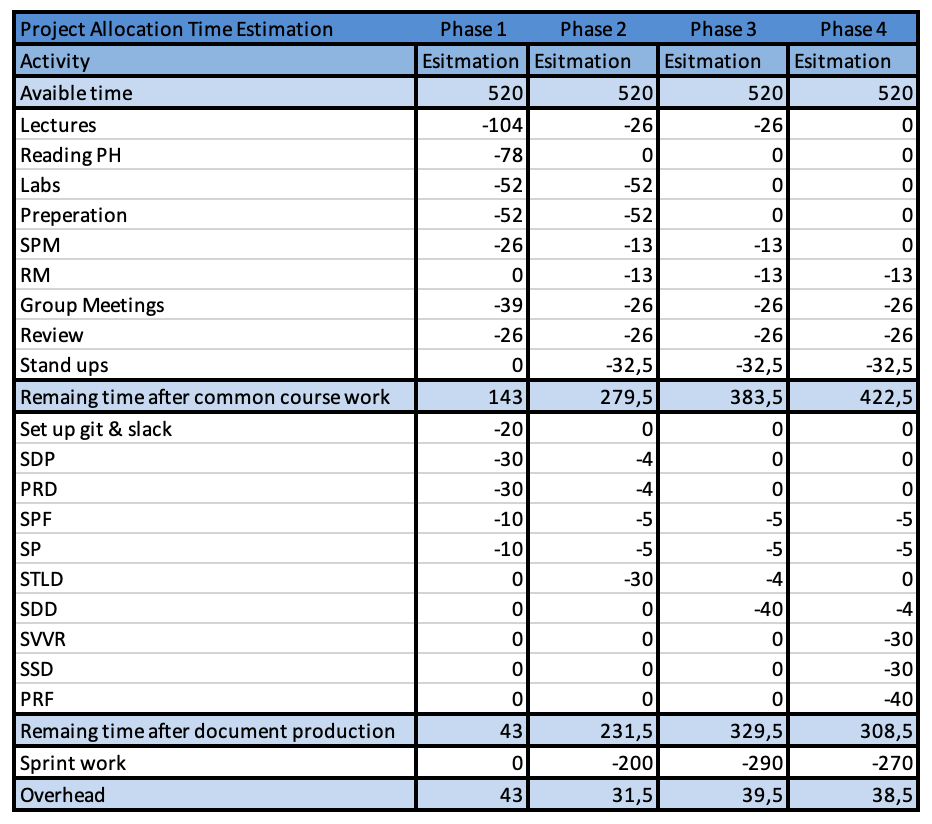
\includegraphics[scale=0.8]{sdpFigures/TimeEst.png}
    \caption{Time allocation estimation for the major events after taking into account other coursework.}
    \label{fig:timeEst}
\end{figure}

\subsection{Gantt Activity chart}
The planning of the main activities of the project, excluding the development of the product, is shown in the Gantt chart in figure \ref{fig:GantAct}.
\begin{figure}[H]
    \centering
    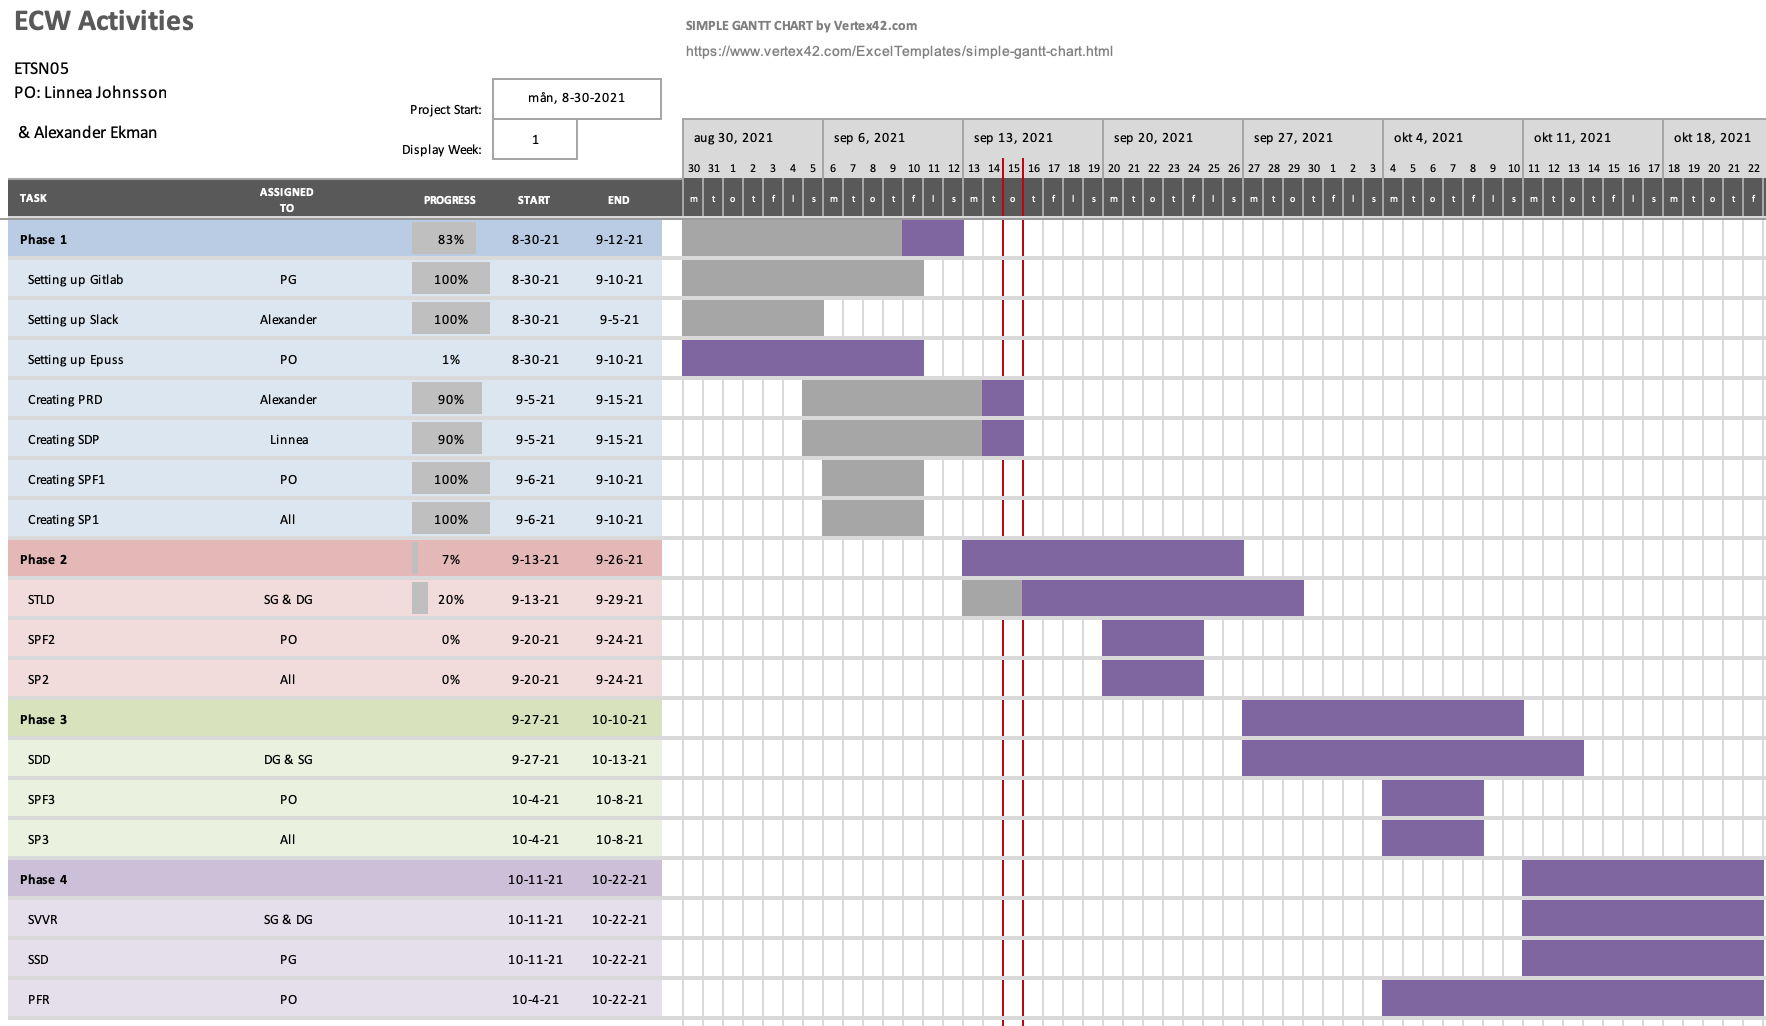
\includegraphics[scale=0.7, angle=90]{sdpFigures/GantActi.png}
    \caption{A Gantt chart over the main activities of the project, besides development.}
    \label{fig:GantAct}
\end{figure}

\subsection{Gantt Development chart}
The time plan for sprint 1 is presented in figure \ref{fig:GantDev}, while the time plan for sprint 1-3 can be viewed in figure \ref{fig:GantDev2}. In the later, the issues had not yet been estimated and could not be placed out. 
\begin{figure}[H]
    \centering
    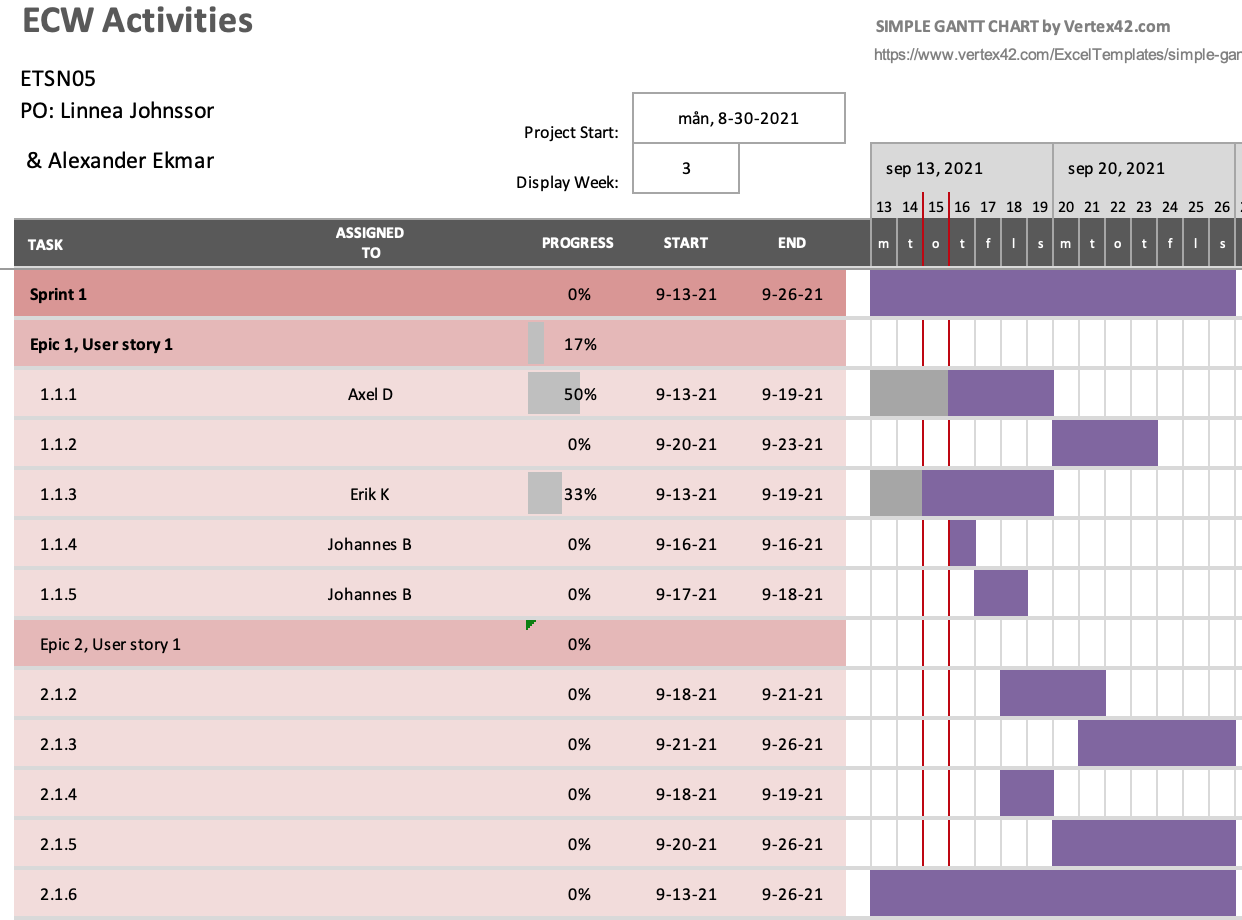
\includegraphics[scale=0.75]{sdpFigures/GantDev.png}
    \caption{A Gantt chart over the development time plan in sprint 1}
    \label{fig:GantDev}
\end{figure}
\begin{figure}[H]
    \centering
    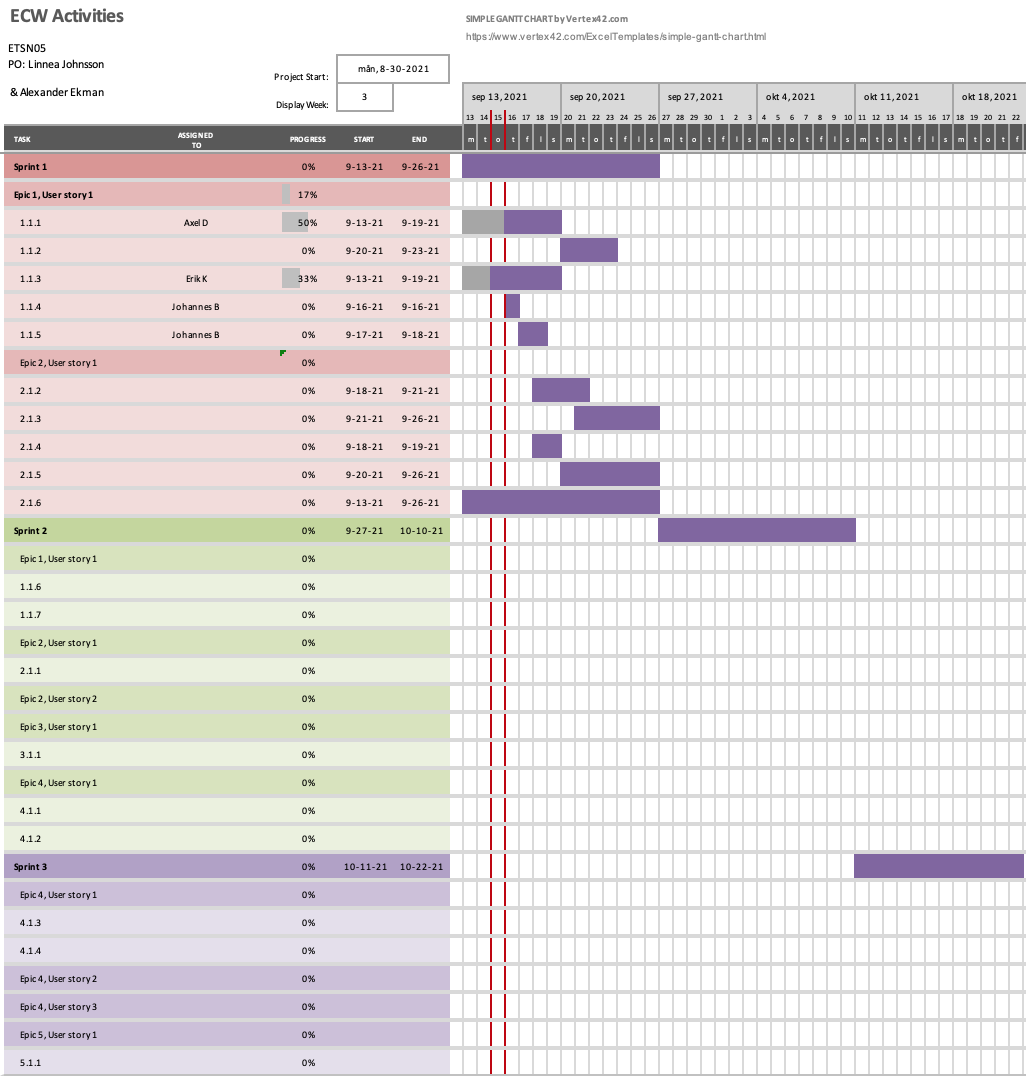
\includegraphics[scale=0.9]{sdpFigures/GantDev2.png}
    \caption{A Gantt chart over the development time plan in all three sprints. For sprints 2-3 estimations had not yet been made the issues could not be scheduled. }
    \label{fig:GantDev2}
\end{figure}

\section{Time plan follow-up and quality review}
The follow-up of the time plan is carried out in three parts. The first part is with measuring the difference between an issue's estimated- and spent time allocation. The second part is using the metric of measuring the number of pushed up and added issues. The pushed up issues only relates to the SP, but the added issues touches both the SPF and the SP. Lastly, a burn down chart and Gantt chart is used to measure the progress in each sprint. 

The quality of the project is measured in two main ways. The first is measuring how well we estimate and plan the different parts of the projects. Secondly, code is reviewed by the SG before merge requests into the main branch are accepted. This is done in order to ensure that the code developed follow the architectural plan of the project. 

\section{Risk analysis}
The risk analysis presented below was made from input from the DG and SG, having the members give input from the point of their area of expertise. I.e. what difficulties they might have run into in prior projects and experiences. 

\subsection{R1}
\textbf{Risk}: Delays\newline
\textbf{Description}: Issues taking longer than estimated\newline
\textbf{Likelihood}: 4/5\newline
\textbf{Severity}: 2/5\newline
\textbf{Indication}: The time plan's overhead grows smaller\newline
\textbf{Prevention}: Overestimate  issues times and have overhead for delays\newline
\textbf{Damage Control}: Pushback other issues to the next sprint or bring in more developers\newline

\subsection{R2}
\textbf{Risk}: Git merge conflicts \newline
\textbf{Description}: Developers working on overlapping code simultaneous creating difficult merge conflicts.  \newline
\textbf{Likelihood}: 4/5\newline
\textbf{Severity}: 1/5\newline
\textbf{Indication}: Bad communication between, and within teams. Few code pushes and far in between. \newline
\textbf{Prevention}: For larger changes in a code file, informing other developers so they do not work simultaneous, i.e. communicating on the Daily stand ups and on the slack channels. \newline
\textbf{Damage Control}: Solve the conflict. \newline

\subsection{R3}
\textbf{Risk}: Absences \newline
\textbf{Description}: Team members getting sick or in other ways not being able to attend to their tasks \newline
\textbf{Likelihood}: 2/5\newline
\textbf{Severity}: 1/5\newline
\textbf{Indication}: No good indications, since sickness and other not planed interference can occur from one day to another. \newline
\textbf{Prevention}: Plan with a lot of overhead. \newline
\textbf{Damage Control}: Reprioritize the SP \newline

\subsection{R4}
\textbf{Risk}: Bugs \newline
\textbf{Description}: Bugs appear in the code and require either refactoring or a online code change. \newline
\textbf{Likelihood}: 4/5\newline
\textbf{Severity}: 1-5/5, depending of type of bug \newline
\textbf{Indication}: If the time spent on reviews and testing is too low.\newline
\textbf{Prevention}: Schedule time for testing and code reviews. \newline
\textbf{Damage Control}: Debug, refactor and/or change the code. \newline

\subsection{R5}
\textbf{Risk}: Changes \newline
\textbf{Description}: Change of specifications late in development  \newline
\textbf{Likelihood}: 2/5\newline
\textbf{Severity}: 5/5 \newline
\textbf{Indication}: Poor communication with client, ambiguous/vague requirements, failure to deliver MVPs in time.\newline
\textbf{Prevention}: Ask if any requirement is unclear, proactively reach out if we find flaws or holes in the current requirements, and/or prototype a solution in the early deliverables and emphasize that we need the customer's thoughts on it.\newline
\textbf{Damage Control}: Delay the project to give time to refactor current designs, documents, code, and test cases. \newline


\end{document}
